\documentclass[bachelor, och, pract, times]{SCWorks}
\usepackage[T2A]{fontenc}
\usepackage[utf8]{inputenc}
\usepackage{graphicx}
\usepackage[sort,compress]{cite}
\usepackage{amsmath}
\usepackage{amssymb}
\usepackage{amsthm}
\usepackage{fancyvrb}
\usepackage{longtable}
\usepackage{array}
\usepackage{pdfpages}

\usepackage[english,russian]{babel}
\usepackage[colorlinks=true]{hyperref}
\begin{document}

% Кафедра (в родительном падеже)
\chair{Дискретной математики и информационных технологий}
% Тема работы
\title{Семейство операционных систем Linux}

% Курс
\course{1}

% Группа
\group{121}

% Факультет (в родительном падеже) (по умолчанию "факультета КНиИТ")
%\department{механико"=математического факультета}

% Специальность/направление код - наименование
%\napravlenie{231000 "--- Фундаментальная информатика и информационные технологии}
%\napravlenie{010500 "--- Математическое обеспечение и администрирование информационных систем}
\napravlenie{09.03.01 "--- Информатика и вычислительная техника}
%\napravlenie{231000 "--- Программная инженерия}
%\napravlenie{090301 "--- Компьютерная безопасность}

% Для студентки. Для работы студента следующая команда не нужна.
%\studenttitle{Студентки}

% Фамилия, имя, отчество студента(ки) в родительном падеже
\author{Давиденко Алексея Алексеевича}

% Заведующий кафедрой
\chtitle{к. ф.-м.н., доцент} % степень, звание
\chname{Л.Б. Тяпаев}  % Инициалы и фамилия

%Научный руководитель (для реферата преподаватель проверяющий работу)
\satitle{к. ф.-м.н., доцент} %должность, степень, звание
\saname{В.А. Поздняков}  % Инициалы и фамилия


% Семестр (только для практики, для остальных
% типов работ не используется)
\term{2} % номер

% Наименование практики (только для практики, для остальных
% типов работ не используется)
\practtype{Учебная практика}

% Продолжительность практики (количество недель) (только для практики,
% для остальных типов работ не используется)
\duration{2} % число недель

% Даты начала и окончания практики (только для практики, для остальных
% типов работ не используется)
\practStart{29.06.2018}  % в формате ДД.ММ.ГГГГ
\practFinish{12.07.2018} % в формате ДД.ММ.ГГГГ

% Год выполнения отчета
\date{2018}  % в формате ГГГГ

\maketitle

% Включение нумерации рисунков, формул и таблиц по разделам
% (по умолчанию - нумерация сквозная)
% (допускается оба вида нумерации)
%\secNumbering


\tableofcontents
\refstepcounter{section}
\refstepcounter{subsection}

\newpage
\subsubsection{Исходный вид статьи}
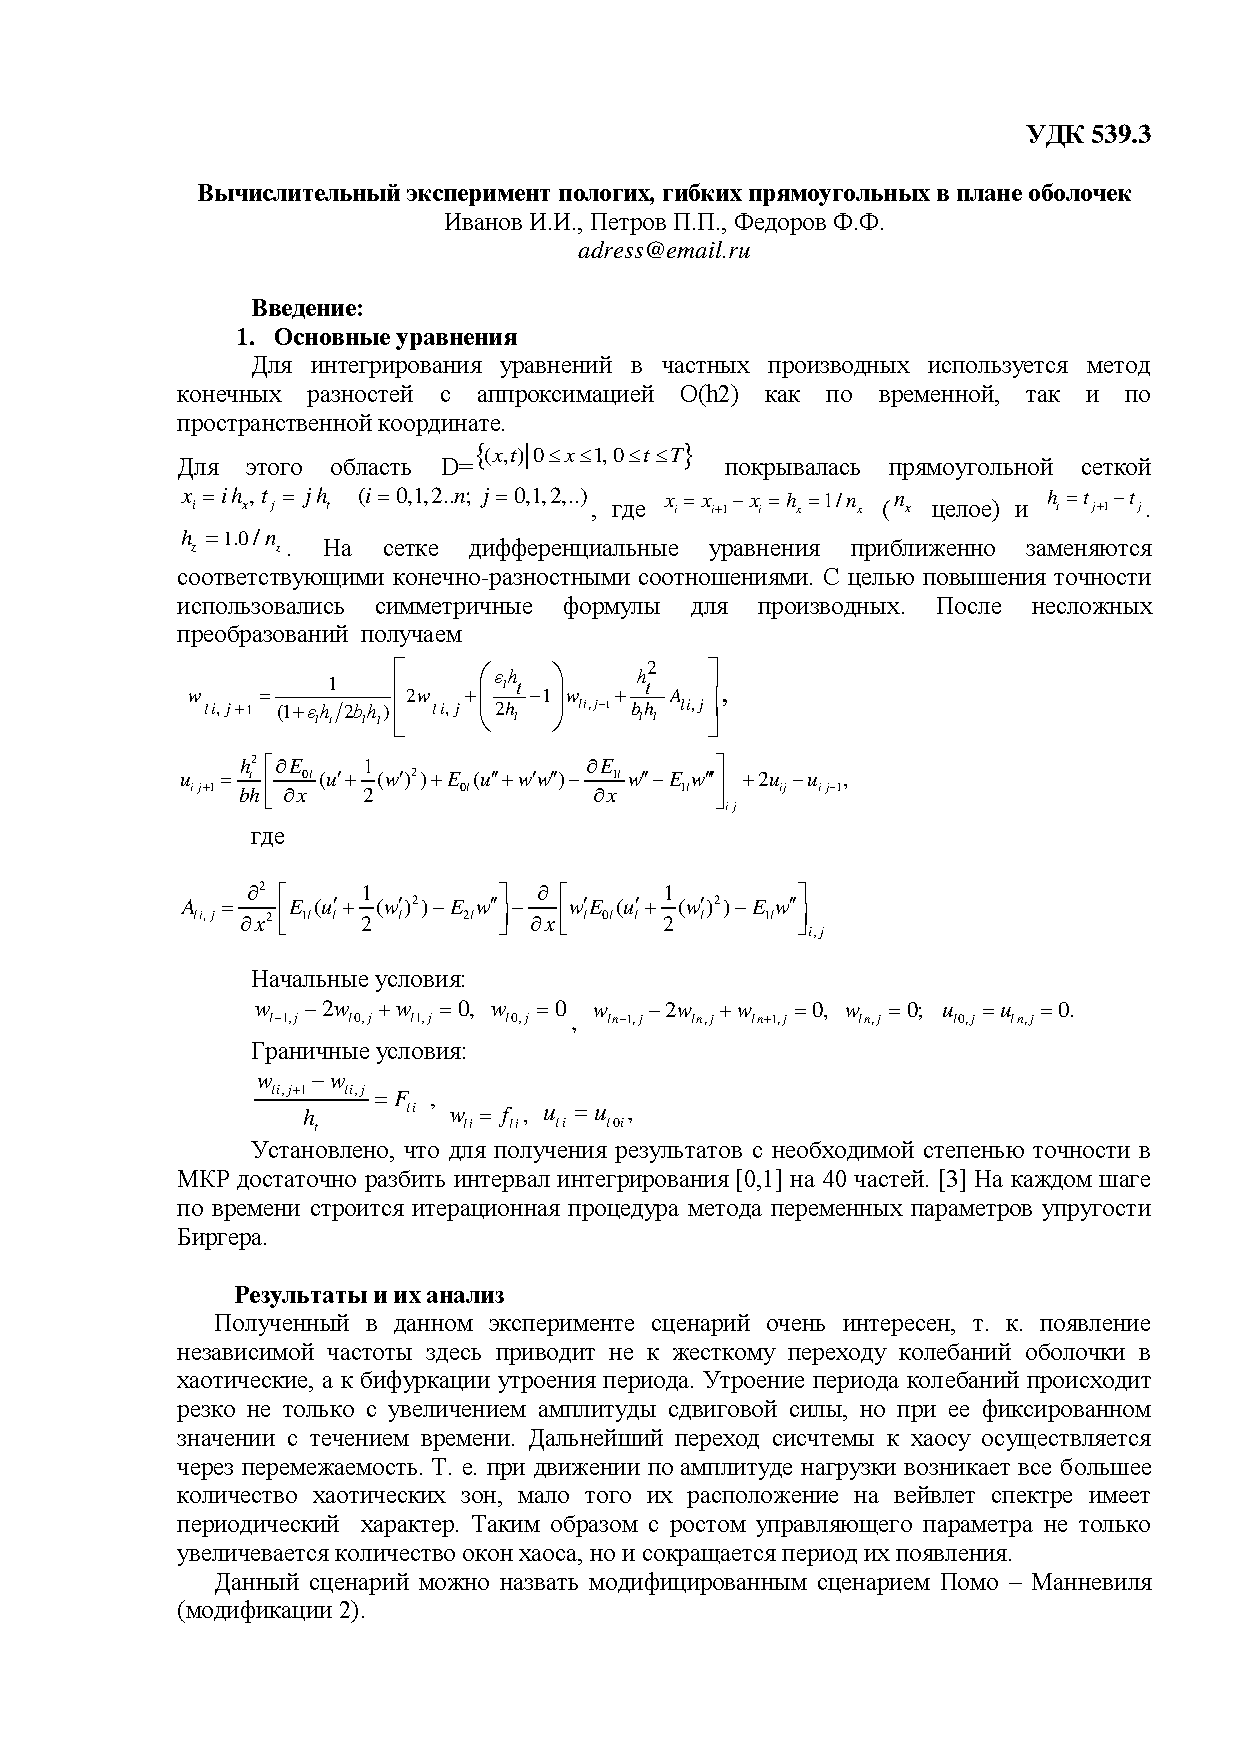
\includepdf[pages=-]{5.pdf}

\subsubsection{Код статьи}
\newpage
\VerbatimInput[fontsize=\small, numbers=left, numbersep=20pt]{ind_zadanie_1.tex}

\newpage
\subsubsection{Свёрстанная статья}
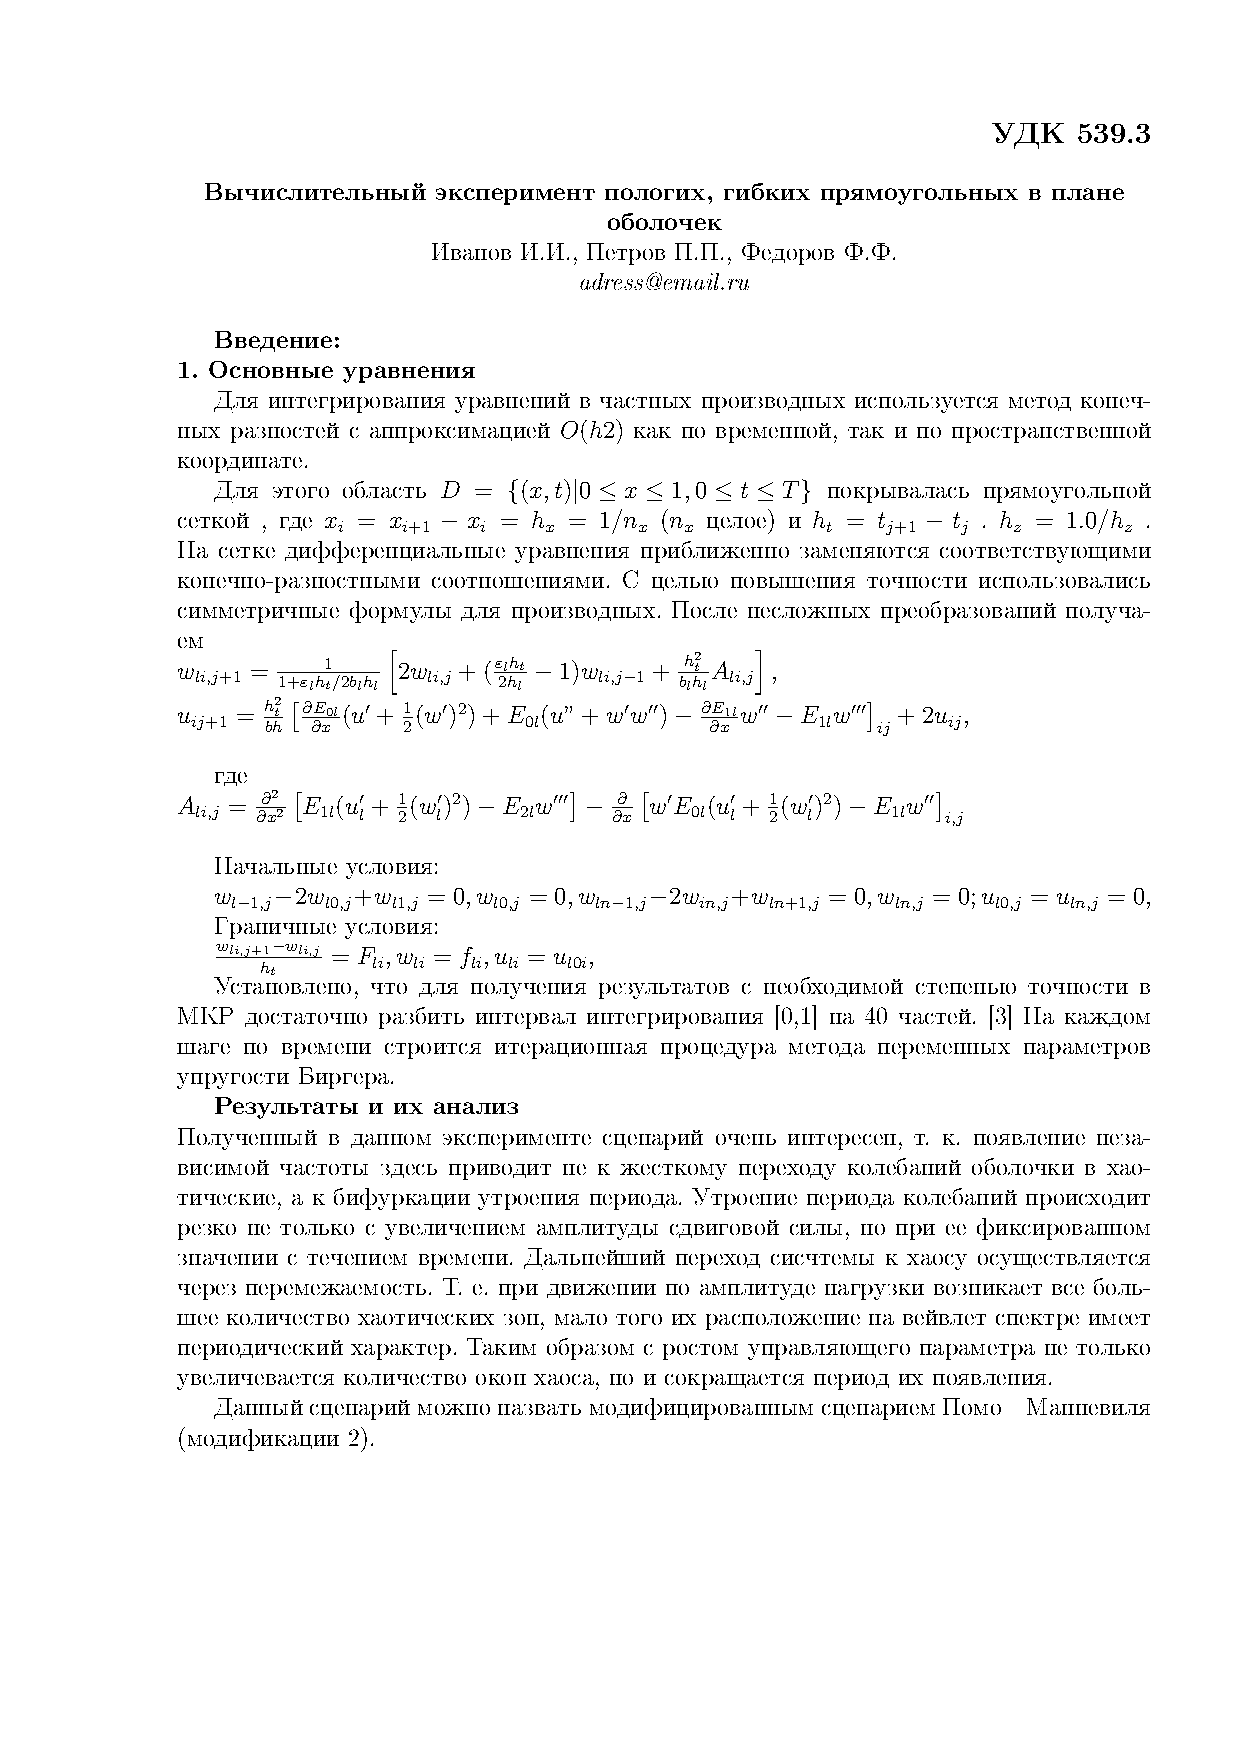
\includepdf[pages=-]{ind_zadanie_1.pdf}

\refstepcounter{subsection}

\subsubsection{Код отчёта}
\newpage
\VerbatimInput[fontsize=\small, numbers=left, numbersep=20pt]{otchet_konf.tex}

\newpage
\subsubsection{Отчёт о посещении конференции}
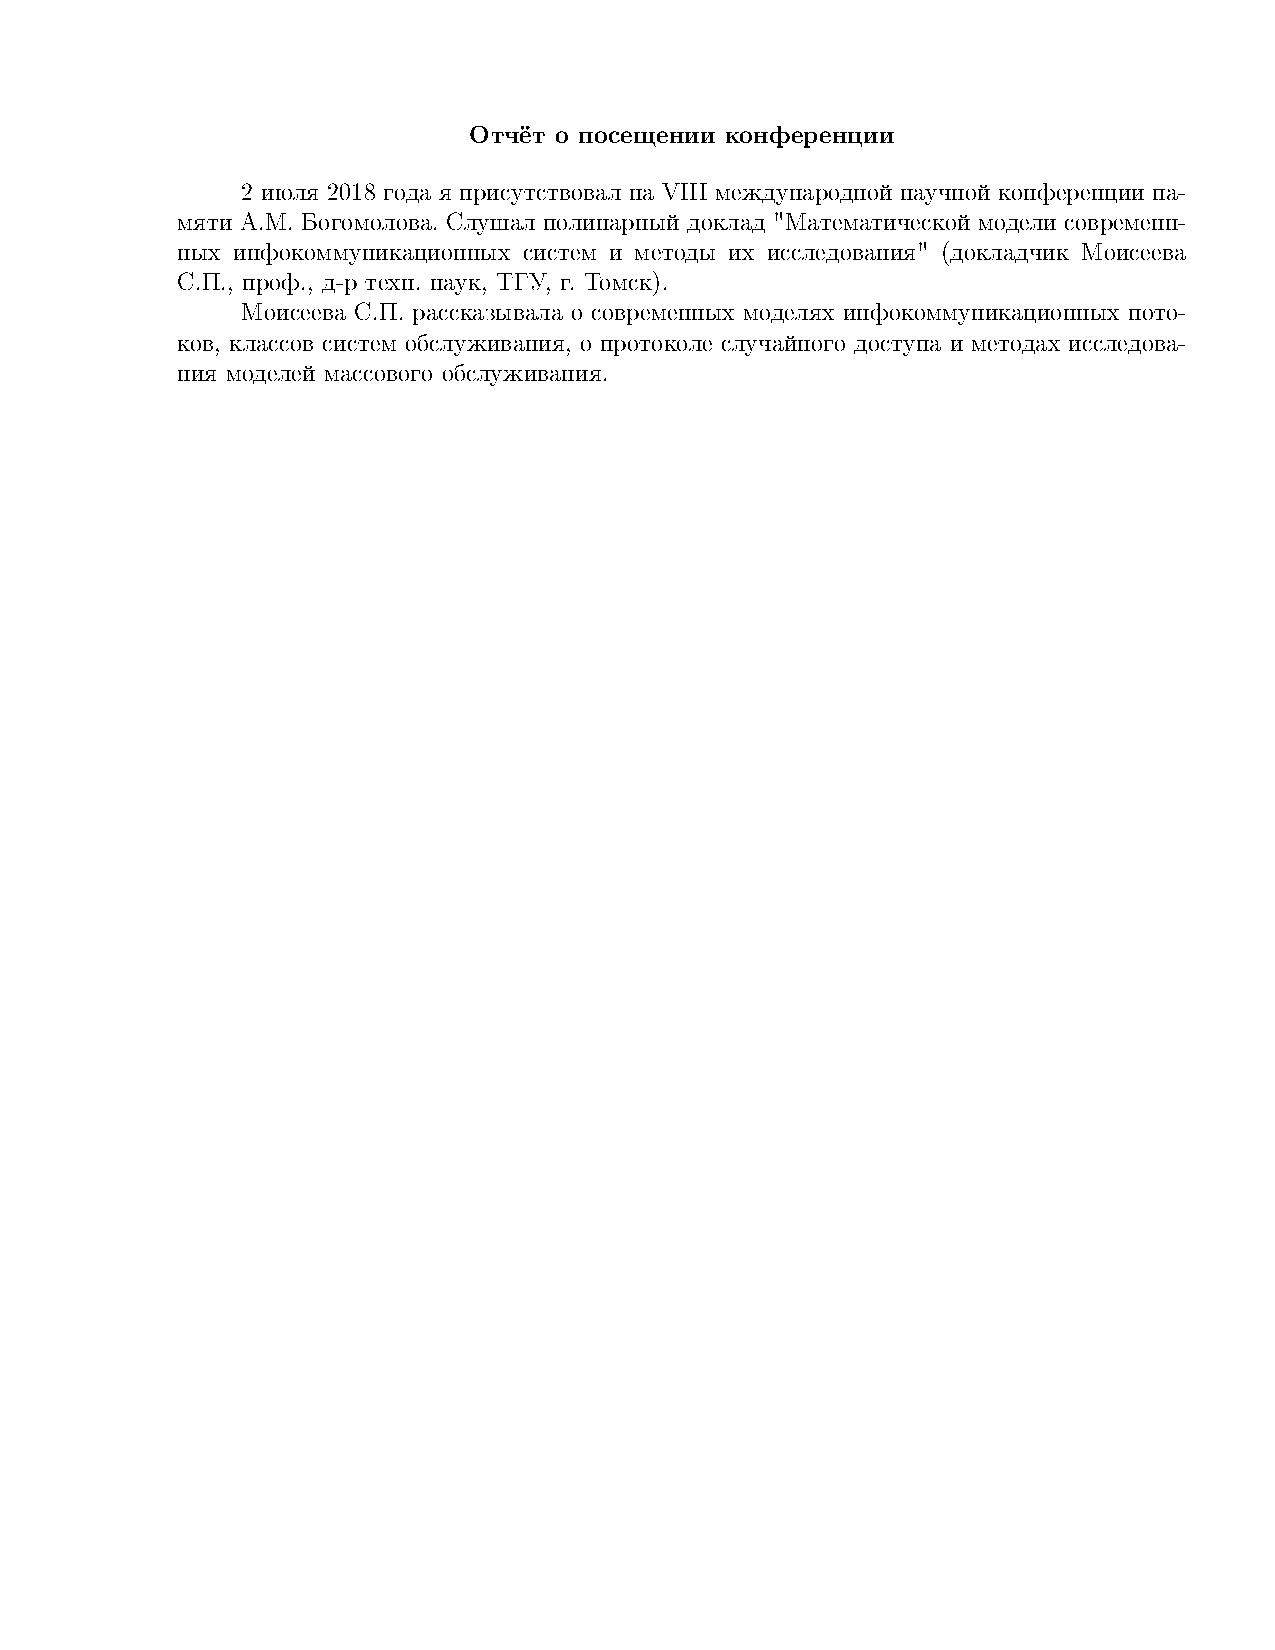
\includepdf[pages=-]{otchet_konf.pdf}

\refstepcounter{section}
\refstepcounter{subsection}

\subsubsection{Код реферата}
\newpage
\VerbatimInput[fontsize=\small, numbers=left, numbersep=20pt]{ind_zadanie_2.tex}

\newpage
\subsubsection{Реферат}

\includepdf[pages=-]{ind_zadanie_2.pdf}


\refstepcounter{subsection}
\subsubsection{Код презентации}
\newpage
\VerbatimInput[fontsize=\small, numbers=left, numbersep=20pt]{pres.tex}

\newpage
\subsubsection{Презентация}

\includepdf[pages=-]{pres.pdf}
\end{document}